\section{Introduction}
\label{sec:intro}

Recent image-to-3D models have made it possible to generate high-quality 3D assets from a single~\cite{Xiang_2025_CVPR_Trellis, Xiang_2026_CVPR_Trellis2,zhao2025hunyuan3d, hunyuan3d2025hunyuan3d, li2025triposg, li2026pixal3d} or multiple views~\cite{chang2026reconviagen, Xiang_2026_CVPR_RnG, shabanov2026free, huang2026unirecgen, schmid2026genrecon}, simplifying 3D content creation and facilitating product visualization or virtual prototyping.
%
Their goal is to reconstruct or generate 3D assets whose geometry and appearance are consistent with the input observations.

However, practical asset creation often requires more than mere reconstruction.
%
For example, a designer may want to modify the proportions of furniture while preserving its distinctive upholstery, or a user may want to reshape a product while retaining its original texture and material.
%
Given multi-view images of a source object and a user-specified target geometry, our goal is to generate a high-quality 3D asset that follows the target shape while retaining the source-specific appearance.
%
We formulate this problem as \emph{geometry-conditioned appearance retargeting} in the image-to-3D generation process.
%
It enables appearance reuse across geometric variations without requiring manual texture editing, which can accelerate 3D asset prototyping and production.

\begin{figure*}[t]
    \centering
    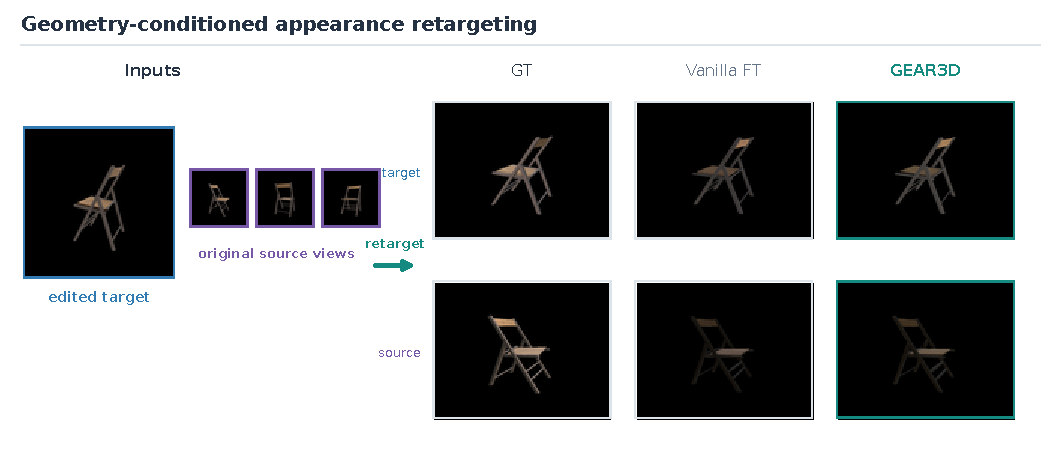
\includegraphics[width=\textwidth]{figures/paper-teaser-v2.pdf}
    \caption{\textbf{Geometry-conditioned appearance retargeting.} An edited
    target view specifies the desired geometry, while three views of the
    original object provide complementary appearance. GEAR3D preserves the
    target-state structure and restores source-specific appearance more
    faithfully than vanilla multi-view fine-tuning in this held-out example.
    Table~\ref{tab:main_quantitative} and the module ablations provide the
    corresponding quantitative evaluation.}
    \label{fig:teaser}
\end{figure*}




\YW{
Despite its practical relevance, this problem presents a challenge distinct from conventional image-to-3D reconstruction.
%
Existing approaches only partially address the requirements of geometry-guided editing.
%
Generating edited multi-view images~\cite{shi2024mvdream, tang2023mvdiffusion, huang2025mv, zhang2026align} can introduce cross-view inconsistencies, while directly deforming a source mesh may produce unintended distortions or artifacts~\cite{yoo2024plausible, choi2026image}.
%
Likewise, modifying geometric latents or applying spatial controls~\cite{fedele2026spacecontrol} may change the geometry without ensuring that the visual condition reflects the edited shape.
%
We therefore employ a geometry-guided vision-language model (VLM) to transform the original target-view image according to a user-specified geometric condition.
%
By leveraging its broad semantic and visual priors, this step expresses diverse geometric modifications as an image-domain target condition compatible with pretrained image-to-3D generation.

However, a geometry-aligned target view alone cannot preserve the object-specific textures and materials, particularly in regions not visible from the target viewpoint.
%
Therefore, we incorporate complementary appearance evidence from the original multi-view source observations.
%
While existing image-to-3D models generally assume that the input observations correspond to the geometry being reconstructed, the edited target and original source images in our setting describe different shapes.
%
Consequently, directly projecting source image features onto the target geometry may associate unrelated surface regions with appearance cues, leading to appearance artifacts and quality degradation.
%
Existing source-aware editing methods~\cite{gat2026shapeup} demonstrate the importance of preserving source appearance, but do not explicitly address this cross-state feature alignment within the 3D generation process.
%
The key challenge is therefore not simply to impose a new geometry, but to \emph{transfer and adapt appearance evidence to the target geometry.}

To this end, we propose \emph{GEAR3D}, a new framework for \emph{\textbf{ge}ometry-conditioned \textbf{a}ppearance \textbf{r}etargeting} in image-to-\textbf{3D} generation that explicitly adapts source-state appearance to the target geometry.
%
Our framework uses the geometry-aligned target view as a structural anchor and incorporates complementary appearance evidence from the original source views.
%
Specifically, we introduce three core modules: (1) \emph{semantic feature matching} to establish correspondences across geometric deformation, (2) \emph{matching-aware feature aggregation} to selectively aggregate source appearance features using ray-shared matching scores, and (3) \emph{target-aware feature retargeting} to adapt the retrieved features to the target state through residual source-feature correction.
%
Furthermore, we construct \emph{DeformNeXt-10k}, a paired deformation dataset with preserved surface correspondences and multi-view observations, to supervise geometry-conditioned appearance retargeting.
}



% Despite its practical relevance, this problem presents a challenge distinct from conventional image-to-3D reconstruction.
% %
% While existing methods generally assume that the input observations correspond to the geometry being reconstructed, the source images and target geometry in our setting describe different shapes.
% %
% Consequently, directly projecting source image features onto the target geometry may associate unrelated surface regions with appearance cues, incurring undesired result and quality degradation.
% %
% Existing approaches only partially address this mismatch.
% %
% Generating edited multi-view images~\cite{shi2024mvdream, tang2023mvdiffusion, huang2025mv, zhang2026align} can introduce cross-view inconsistency, directly deforming a source mesh often produces unintentional distortions or artifacts~\cite{yoo2024plausible, choi2026image}, and solely modifying geometric latents~\cite{fedele2026spacecontrol} or directly reusing original image features~\cite{gat2026shapeup} may lead to a misalignment between visual features and the target 3D state.
% %
% The key challenge is therefore not simply to impose a new geometry, but to \emph{transfer and adapt appearance evidence to the target geometry.}



% To this end, we propose \emph{GEAR3D}, a new framework for \emph{\textbf{ge}ometry-conditioned \textbf{a}ppearance \textbf{r}etargeting} for image-to-\textbf{3D} generation, that explicitly models source-state appearance according to target-state geometry.
% %
% Our framework establishes a geometry-aligned target view as the structural anchor and incorporates complementary appearance evidence from the original source views.
% %
% Specifically, we introduce three core modules: (1) \emph{semantic feature matching} to establish correspondences across geometric deformation, (2) \emph{matching-aware attention} to selectively retrieve appearance features from corresponding source regions, and (3) \emph{deformation-aware feature retargeting} to adapt the retrieved features to the target geometry.
% %
% Furthermore, we construct DeformNeXt-10k, a paired deformation dataset with preserved surface correspondences and multi-view observations, to supervise geometry-conditioned appearance retargeting.






Our main contributions are summarized as follows:

\YW{
\begin{itemize}
    \item We formulate \emph{geometry-conditioned appearance retargeting} to adapt source appearance to the target geometry.

    \item We propose a target-anchored 3D generative framework combining \emph{semantic feature matching}, \emph{matching-aware feature aggregation}, and \emph{target-aware feature retargeting} to align, retrieve, and adapt source appearance evidence.

    \item We construct \emph{DeformNeXt-10k}, a paired deformation dataset with surface correspondences and multi-view observations, for systematic training and evaluation.
\end{itemize}
}

% \begin{itemize}
%     \item We formulate geometry-conditioned appearance retargeting, where source images and target geometry intentionally describe different geometry, requiring appearance transfer and adaptation across geometric variations.
%     % \item We introduce a target-anchor formulation that separates target-state geometry from source-state appearance evidence, enabling the use of complementary source views without enforcing their outdated geometry.
%     \item We propose a novel target-anchored 3D generative framework with semantic feature matching, matching-aware attention, and deformation-aware feature retargeting to align, retrieve, and adapt source appearance evidence.
%     % \item We propose semantic feature matching, matching-aware attention, and deformation-aware feature retargeting to respectively establish correspondence, route source evidence, and adapt it to the target geometry.
%     \item We construct DeformNeXt-10k, comprising 10,165 paired deformations with surface correspondences, to support supervised learning and evaluation of geometry-conditioned appearance retargeting.
% \end{itemize}
